%% bpmlr.tex
%% V0.1
%% 2015/01/01
%% by Mack Sweeney

\documentclass[10pt]{proc}


% *** CITATION PACKAGES ***
%
\usepackage{cite}

% *** OTHER BIBLIOGRAPHY PACKAGES ***
%
%\usepackage[numbers]{natbib}


% *** GRAPHICS RELATED PACKAGES ***
%
\usepackage[pdftex]{graphicx}
% declare the path(s) where your graphic files are
\graphicspath{{./graphics/}}
% and their extensions so you won't have to specify these with
% every instance of \includegraphics
\DeclareGraphicsExtensions{.pdf,.jpeg,.png}

\usepackage{scalerel}
\usepackage{mdframed}

% For graphical models:
\usepackage{tikz}
\usetikzlibrary{bayesnet}


% *** MATH PACKAGES ***
%
\usepackage[cmex10, fleqn]{amsmath}
\usepackage{bm}
\usepackage{bbm}
\usepackage{amssymb}
\usepackage{mathtools}
\usepackage{etoolbox}
%
% Also, note that the amsmath package sets \interdisplaylinepenalty to 10000
% thus preventing page breaks from occurring within multiline equations. Use:
\interdisplaylinepenalty=2500
% after loading amsmath to restore such page breaks as IEEEtran.cls normally
% does. amsmath.sty is already installed on most LaTeX systems.


% *** SPECIALIZED LIST PACKAGES ***
%
\usepackage{algorithm}
\usepackage[noend]{algpseudocode}


% *** ALIGNMENT PACKAGES ***
%
\usepackage{array}
\usepackage{booktabs}


% *** SUBFIGURE PACKAGES ***
%\usepackage[tight,footnotesize]{subfigure}
%\usepackage[caption=false]{caption}
%\usepackage[font=footnotesize]{subfig}
\usepackage[caption=false,font=footnotesize]{subfig}


% *** FLOAT PACKAGES ***
%
%\usepackage{fixltx2e}
\usepackage{stfloats}


% *** PDF, URL AND HYPERLINK PACKAGES ***
%
\usepackage{url}


% BEGIN PAPER CONTENT
%
\title{Infinite Profiling Mixtures of Linear Regressions}
\author{
    Mack Sweeney, Kathryn Laskey, Huzefa Rangwala\\
        George Mason University
}
\date{\today}


% New commands to be used in this report.
\newcommand*{\Scale}[2][4]{\scalebox{#1}{$#2$}}%
\newcommand*{\Resize}[2]{\resizebox{#1}{!}{$#2$}}%
\newcommand{\norm}[1]{\left\lVert#1\right\rVert}
\newcommand{\pluseq}{\mathrel{+}=}
\newcommand{\mineq}{\mathrel{-}=}
\newcommand{\asteq}{\mathrel{*}=}
\newcommand{\elips}[1]{\ldots#1\allowbreak}
\newcommand{\bc}{,\allowbreak}
\newcommand*\diff{\mathop{}\!\mathrm{d}}

\AtBeginEnvironment{align}{\par\small}
\AfterEndEnvironment{align}{\normalsize}
\AtBeginEnvironment{align*}{\par\small}
\AfterEndEnvironment{align*}{\normalsize}
\AtBeginEnvironment{flalign}{\par\small}
\AfterEndEnvironment{flalign}{\normalsize}
\AtBeginEnvironment{algorithmic}{\par\small}
\AfterEndEnvironment{algorithmic}{\normalsize}

\newtheorem{lemma}{Lemma}
\newtheorem{proof}{Proof}


\begin{document}
\maketitle


\begin{abstract}

\end{abstract}


\section{Introduction}

Navigating a university degree program is a duanting task. There are often
several categories of requirements that need to be met, each with several
courses to choose from. Students wish to choose courses that will meet these
requirements. They also want to avoid taking courses so difficult they are
unable to learn the material and perform well.

This selection task is complicated by the fact that students take multiple
courses each semester. Taking one particularly difficult course may be an
exciting challenge, while taking two or three concurrently would be
overwhelming. So there is a need to properly blend courses of varying difficulty
in a single semester. Certain course combinations may also be very
complementary. For instance, many courses are associated with labs, which
provide practical experience with the theoretical lecture concepts.

The selection task is also complicated by the sequential nature of learning.
Many courses build upon knowledge learned in previous courses. Some courses can
only be taken if the student has already taken the prerequisite courses. Other
courses do not have these requirements but should still not be taken unless
certain prerequisite knowledge has been learned. If no prerequisites are given,
students must determine for themselves which prior courses should have been
taken in order to do well in a course currently being selected.

Beyond the questions of difficulty and requirements, students would also like to
explore their individual interests as much as possible. With all else being
equal between two courses, the student will choose the most interesting one.
Sometimes personal interest will also lead students to take a course which is
more difficult but meets the same requirement as an easier course. This
subjective factor makes it impossible for a one-size-fits-all course selection
to be successful.

We seek to address one particular aspect of the degree planning problem
described above. We seek to assist students in ranking courses for a particular
semester given all prior course data for all students in the university. In this
study, we rank these courses based on student-relative difficulty

\section{Problem Formulation}\label{problem-formulation}

In the traditional university setting, cohorts of students are admitted and
begin taking courses. Each semester, students can enroll in zero or more courses
and earn grades in each course. These grades are assigned on a 0-100 scale. At
the end of the course, the final grades are binned into categorical values on
the A-F scale (A, A-, B+, B, ..., C, C-, D, F). These categorical values are
often mapped to a numerical categorical scale of 4-0 for grade point average
(GPA) calculations.

Our dataset consists of polyadic relationships resulting from students taking
courses over a sequence of semesters. Each record is uniquely identified by the
student id (sid), course id (cid), and a chronological semester number (term).
We can organize these triads into a sparse tensor $\bm{Y} \in \mathbb{R}^{N
\times M \times T}$. $N$ is the number of unique students in the dataset,
$M$ the number of unique courses, and $T$ the number of terms. So entry
$\bm{Y}_{n,m,t} \in [0, 4]$ represents the grade student $n$ earned in course
$m$ during semester $t$. These grades are ordinal values in the range 0 to 4.

We also observe various pieces of \textit{side information} for each observed triad.
Side information includes observations aside from the grade that describe the
entities of the triad (student, course, term) or their interaction.  For
instance, student side information includes demographics. Course side info
includes attributes of the instructor. Term side info might include
university-wide statistics from that term or previous terms. Side info
describing interactions is rich and diverse. Two examples are the number of
credit hours a student is enrolled in during the term and a student's past
performance in all courses of the same discipline. We extract $f$ features from
the side info and assemble it into a sparse tensor $\bm{X} \in \mathbb{R}^{n
\times m \times t \times f}$.

We often want to split our database into train and test sets. We assume
the train set is unobserved and make predictions about the unobserved test set.
For this purpose, we define $Y^{(t)}$ to be the cumulative grade matrix up to
and including term $t$. We define this recursively:
%
\begin{enumerate}
    \item  $Y^{(0)} = \bm{Y}_{*,*,0}$
    \item  $Y^{(t)} = join(Y^{(t-1)}, \bm{Y}_{*,*,t})$,
\end{enumerate}
%
where $join$ is an inner-join on the (cid, sid, term) fields. Conflicts are
resolved by keeping the values from the more recent term. We define
$\bm{X}^{(t)}$ to be the cumulative feature vector matrix, recursively
accumulated in the same manner. Throughout the paper, we assume we are
currently in term $t$ and have been given data for terms up to $t-1$. We leave
off the term superscript, so $Y$ represents $Y^{(t-1)}$ and $\bm{X}$ represents
$\bm{X}^{(t-1)}$. Finally, we define $\bm{D} = (\bm{X}, Y)$ to be the observed
data.

Given the cumulative grades $Y$ and feature vectors $\bm{X}$, our task is to
predict the unobserved grades in term $t$.

\section{Notation}

\subsection{Data}

{\footnotesize
\begin{tabular}{p{0.35\columnwidth} p{0.6\columnwidth}}
    $N$         &   Number of students.     \\
    $M$         &   Number of courses.      \\
    $T$         &   Number of semesters.    \\
    $f$         &   Number of features.     \\
    $\bm{X} \in \mathbb{R}^{N \times M \times T \times f}$
                &   Tensor of observed feature vectors. \\
    $\bm{Y} \in \mathbb{R}^{N \times M \times T}$
                &   Tensor of observed ordinal grades.  \\
    $\bm{D}_{nm} = (\bm{X}_{nm}, \bm{Y}_{nm})$
                &   All observed data for student $n$, course $m$.  \\
\end{tabular}}

\subsection{Model Parameters}

{\footnotesize
\begin{tabular}{p{0.3\columnwidth} p{0.6\columnwidth}}
    $K$                         &   Number of components in finite mixture model. \\
    $Z_{n} = \{1, ..., K\}$     &   Discrete latent state indicating which
                                    component $\bm{D}_{nm}$ belongs to.           \\
    $\bm{\pi}_k = P(Z_n = k)$   &   Prior probability $\bm{D}_{nm}$ is assigned
                                    to mixture component $k$.                     \\
    $\bm{w_k}$          &   Regression coefficients (and mean vector)
                            for component $k$.                                    \\
    $\sigma_k^2$        &   Regression variance for component $k$.                \\
    $G_{nm}$            &   Latent real-valued grade of student $n$ in course $m$.\\
    $\bm{s}_n$          &   bias term for student $n$.                            \\
    $\bm{c}_m$          &   bias term for course $m$.                             \\
\end{tabular}}

\subsection{Hyper-parameters}

{\footnotesize
\begin{tabular}{p{0.35\columnwidth} p{0.6\columnwidth}}
    $\alpha$                    &   Dirichlet concentration parameter           \\
    $\Theta= (\bm{w}_0, \kappa_0, \alpha_0, \beta_0)$
                    &   Parameters for the Guassian-Inverse-Gamma
                        ($\mathcal{N}\Gamma^{-1}$) prior on mean vector $\bm{w}_k$ and
                        variance $\sigma_k^2$ of a multivariate Gaussian distribution.
                        Interpretations for each are given below.               \\
    $\bm{w}_0$      &   Prior mean of $\bm{w}_k$                                \\
    $\kappa_0$      &   How strongly we believe the $\bm{w}_0$ prior            \\
    $\alpha_0$      &   Shape parameter for $\Gamma^{-1}$ prior on $\sigma_k^2$ \\
    $\beta_0$       &   Rate parameter for $\Gamma^{-1}$ prior on $\sigma_k^2$  \\
    $\Theta_s = (\mu_s, \sigma_s^2)$
                    &   Mean and variance for the Guassian prior on $s_n$       \\
    $\Theta_c = (\mu_c, \sigma_c^2)$
                    &   Mean and variance for the Gaussian prior on $c_m$       \\
\end{tabular}}


\section{Modeling}\label{model}

We build a model that (1) accurately predicts next-term grades given data from
previous terms, (2) clusters students to identify common learner profiles, and
(3) is highly interpretable. We derive a fully Bayesian probabilistic model that
combines mixtures of linear regressions with nonparametric model selection.

We start with the familiar Finite Gaussian Mixture Model (GMM) with $K$
components. Then we slowly mutate the model to introduce additional data
relevant to the next-term grade prediction problem. Finally we arrive at the
Personalized Mixture of Linear Regressions for Ordinal data (PMLRO).

We define $\mathbb{C} = (1, ..., m)$ to be the set of all course IDs. We also
define a function random-subset($\mathbb{C}$) that takes a set and returns a
small random subset of it. $\mathcal{N}_f$ is the f-dimensional multivariate
Gaussian and $\mathcal{W}^{-1}$ is the inverse-Wishart distribution.
Algorithm~\ref{alg:gmm-genp} lays out the generative process for the feature
vectors $\bm{X}$.
%
\begin{algorithm}
    \caption{GMM Generative Process for $\bm{X}_{nm}$}
    \label{alg:gmm-genp}
    \begin{algorithmic}[1]
        \item  Draw $\bm{\pi} \sim \text{Dir}(\alpha)$.
        \For{$k$ in $1..K$}
            \State  Draw $\Sigma_k \sim \mathcal{W}^{-1}(\nu_0, \Sigma_0)$.
            \State  Draw $\bm{\mu}_k \sim
                \mathcal{N}_f(\bm{\mu_0}, \frac{1}{\kappa_0}\Sigma_k)$.
        \EndFor
        \For{$n$ in $1..N$}
            \State  Draw $Z_n \sim \text{Mult}(\bm{\pi}_1, ..., \bm{\pi}_k)$.
            \For{$m$ in random-subset($\mathbb{C}$)}
                \State  Draw $\bm{X}_{nm} | Z_n \sim \mathcal{N}_f(\bm{\mu}_k, \Sigma_k)$.
            \EndFor
        \EndFor
    \end{algorithmic}
\end{algorithm}
%
This is the standard conjugate GMM, which corresponds to the graphical model
shown in Figure~\ref{fig:gmm-pgm}.

% GMM PGM
\begin{figure}[tbh]
  \setlength{\belowcaptionskip}{15pt plus 3pt minus 2pt}
  \centering
  \caption{Finite Gaussian Mixture Model. The hyper-parameters
           $\Theta = (\mu_0, \kappa_0, \nu_0, \Sigma_0)$. }
  \label{fig:gmm-pgm}
  \scalebox{0.9}{
  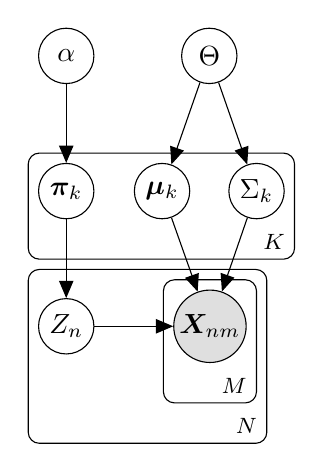
\begin{tikzpicture}

    % Define nodes
    \node[obs]                                (X) {$\bm{X}_{nm}$};
    \node[latent, left=of X]                  (Z) {$Z_n$};
    \node[latent, above=of Z]                (pi) {$\bm{\pi}_k$};
    \node[latent, above=of pi]            (alpha) {$\alpha$};
    \node[latent, right=of alpha, xshift=0.1cm]  (theta) {$\Theta$};

    \node[latent, below=of theta, xshift=-0.6cm] (mk) {$\bm{\mu}_k$};
    \node[latent, below=of theta, xshift=0.6cm]  (sk) {$\Sigma_k$};

    % Connect the nodes
    \edge {Z} {X};
    \edge {pi} {Z};
    \edge {alpha} {pi};
    \edge {theta} {mk,sk};
    \edge {mk,sk} {X};

    % Plates
    \plate {course} {(X)} {$M$};
    \plate {student}%
           {(Z)(X)(course.south east)(course.north east)(course.north west)}%
           {$N$};
    \plate {comps} {(pi)(mk)(sk)} {$K$};

  \end{tikzpicture}}
\end{figure}

This model clusters the students based on the features from each of the courses
taken. However, it is not able to predict grades, since the grades are not
included in the model. We next extend the model to a mixture of Gaussian linear
regressions with coefficients $W \in \mathbb{R}^{K \times f}$ and
variances $\bm{\sigma}_k^2$. We say that each grade is produced by linear
regression $k$ with probability $\bm{\pi}_k$.
%
\begin{align}
    G_n =
    \begin{cases}
        \bm{X}_n W_1 + \epsilon_1  &  \text{with probability } \bm{\pi}_1  \\
        \bm{X}_n W_2 + \epsilon_2  &  \text{with probability } \bm{\pi}_2  \\
        ...                        &                                       \\
        \bm{X}_n W_k + \epsilon_k  &  \text{with probability } \bm{\pi}_k
    \end{cases}
\end{align}
%
The error term $\epsilon_k$ is assumed to be 0-centered Gaussian noise:
$\epsilon_k \sim \mathcal{N}(0, \bm{\sigma}_k^2)$. This model yields the following
mixture of multivariate normals:
%
\begin{align}
    G_n &\sim
        \sum_{k=1}^K \bm{\pi}_k
            \mathcal{N}(\bm{X}_n W_k, I \bm{\sigma}_k^2)  \\
    G_n | Z_n &\sim
        \mathcal{N}(\bm{X}_n W_k, I \bm{\sigma}_k^2)
\end{align}
%
We place a conjugate Gaussian-Inverse-Gamma (GIG) prior on $W_k,
\bm{\sigma}_k^2$ (WE CAN ALSO CONSIDER IMPROPER PRIORS WHICH LEAD TO THE
CLASSICAL LEAST SQUARES ESTIMATES):
%
\begin{align}
    \bm{\sigma}_k^2 &\sim \text{IG}(\alpha_0, \beta_0),  \\
    W_k | \bm{\sigma}_k^2 &\sim
        \mathcal{N}(\mu_0, V_0 \bm{\sigma}_k^2),
\end{align}
%
This gives us the model shown in Figure~\ref{fig:mglr-pgm}. We call this model
the Mixture of Gaussian Linear Regressions (MGLR).
Algorithm~\ref{alg:mglr-genp} summarizes the grade generation process under
MGLR.
%
\begin{algorithm}
    \caption{MGLR Generative Process for $G_n$}
    \label{alg:mglr-genp}
    \begin{algorithmic}[1]
        \item  Draw $\bm{\pi} \sim \text{Dir}(\alpha)$.
        \For{$k$ in $1..K$}
            \State  Draw $\bm{\sigma}_k^2 \sim \text{IG}(\alpha_0, \beta_0)$.
            \State  Draw $W_k \sim
                \mathcal{N}_f(\bm{\mu_0}, V_0 \bm{\sigma}_k^2)$.
        \EndFor
        \For{$n$ in $1..N$}
            \State  Draw $Z_n \sim \text{Mult}(\bm{\pi}_1, ..., \bm{\pi}_k)$.
            \For{$m$ in random-subset($\mathbb{C}$)}
                \State  Draw $G_{nm} | Z_n, \bm{X}_{nm} \sim
                    \mathcal{N}_f(\bm{X}_{nm} W_k, \bm{\sigma}_k^2)$.
            \EndFor
        \EndFor
    \end{algorithmic}
\end{algorithm}

The resulting posterior distribution is:
%
\begin{align}
    P(W_k, \bm{\sigma}_k^2) &\sim
        \mathcal{N}(\mu^*, \bm{\sigma}_k^2 V_0)
        \text{IG}(\alpha^*, \beta^*),
\end{align}
%
where
%
\begin{flalign}
    \bm{\mu}^* &= \left[
        V_0^{-1} + \bm{X}_n^T \bm{X}_n
    \right]^{-1}  \left[
        V_0^{-1} \bm{\mu_0} + \bm{X}_n^T G_n
    \right]  \\
%%
    V^* &= \left[
        V_0^{-1} + \bm{X}_n^T \bm{X}_n
    \right]^{-1}  \\
%%
    \alpha^* &= \alpha_0 + n / 2  \\
%%
    \beta^* &= \beta_0 + \frac{1}{2}\left(
        G_n^2
        + \bm{\mu_0}^T V_0^{-1} \bm{\mu_0}
        - \bm{\mu}^{*T} V^{*-1} \bm{\mu}^*
    \right)
\end{flalign}

Our goal is to use this model to predict grades. If the parameters $W$ and
$\bm{\sigma}^2$ were known, the probability of the grades conditional on known
component membership would be
$G_n | Z_n, W, \bm{\sigma}^2 \sim \mathcal{N}(X_n W_k, I \bm{\sigma}_k^2)$.
Since we don't know these parameters, they must be summarized through their
posterior samples. Therefore all predictions must come from the
\textit{posterior predictive distribution}, which is a multivariate $t$
distribution. Given the posterior parameters $\Theta^* = (\bm{\mu^*}, V^*,
\alpha^*, \beta^*)$, we have:
%
\begin{align}
    &P(G_n | \bm{D})  \nonumber \\
     &= \int \mathcal{N}(X_n W_k, \bm{\sigma}_k^2)
             \text{GIG}(\Theta^*)
             \diff W_k \diff \bm{\sigma}_k^2 \\
     &= MVSt_{\nu^*} \left(
            X_n \bm{\mu^*},
            \frac{\beta^*}{\alpha^*}(I + X_n V^* X_n^T)
        \right)
\end{align}

This works only if we know the component $Z_n = k$ with certainty. These
latent parameters are inferred from the data. So we must also incorporate this
uncertainty when making predictions. Given $W$ and $\bm{\sigma}_k^2$ we can
compute an MLE of the posterior component membership weights $\bm{\pi}^*$:
%
\begin{align}
    M_{nk} &= p(Z_n = k | \bm{D}_n, W, \bm{\sigma}_k^2) p(Z_n = k)    \\
           &\propto \mathcal{N}(X_n W_k, \bm{\sigma}_k^2) \bm{\pi}_k  \\
    \bm{\pi}_k^* &= \frac{1}{N} \sum_{n=1}^N M_{nk}
\end{align}
%
With these weights, we can compute the posterior predictive with unknown
indicator variables:
%
\begin{align}
    &P(G_n | \bm{D})  \nonumber \\
     &= \int \sum_{k=1}^K \bm{\pi}_k
            \mathcal{N}(X_n W_k, \bm{\sigma}_k^2)
                 \text{GIG}(\Theta^*)
                 \diff W_k \diff \bm{\sigma}_k^2 \\
     &= \sum_{k=1}^K \bm{\pi}_k^*
            MVSt_{\nu^*} \left(
                X_n \bm{\mu^*},
                \frac{\beta^*}{\alpha^*}(I + X_n V^* X_n^T)
        \right)
\end{align}

% Mixture of Gaussian Linear Regressions (MGLR) PGM
\begin{figure}[tbh]
  \setlength{\belowcaptionskip}{15pt plus 3pt minus 2pt}
  \centering
  \caption{Finite Mixture of Guassian Linear Regressions. The hyper-parameters
           $\Theta = (\mu_0, V, \alpha_0, \beta_0)$. }
  \label{fig:mglr-pgm}
  \scalebox{0.9}{
  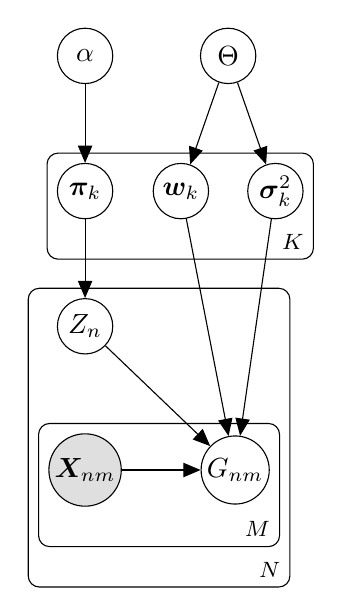
\begin{tikzpicture}

    % Define nodes
    \node[obs]                                (X) {$\bm{X}_{nm}$};
    \node[latent, right=of X]                 (G) {$G_{nm}$};
    \node[latent, above=of X]                 (Z) {$Z_n$};
    \node[latent, above=of Z]                (pi) {$\bm{\pi}_k$};
    \node[latent, above=of pi]            (alpha) {$\alpha$};
    \node[latent, right=of alpha, xshift=0.1cm] (theta) {$\Theta$};

    \node[latent, below=of theta, xshift=-0.6cm] (mk) {$\bm{w}_k$};
    \node[latent, below=of theta, xshift=0.6cm]  (sk) {$\bm{\sigma}_k^2$};

    % Connect the nodes
    \edge {Z,X,mk,sk} {G};
    \edge {pi} {Z};
    \edge {alpha} {pi};
    \edge {theta} {mk,sk};

    % Plates
    \plate {course} {(X)(G)} {$M$};
    \plate {student}%
           {(Z)(X)(G)(course.south east)(course.north east)(course.north west)}%
           {$N$};
    \plate {comps} {(pi)(mk)(sk)} {$K$};

  \end{tikzpicture}}
\end{figure}

With the MGLR model, we can predict student grades using linear relationships
with the covariates. We also obtain a probabilistic clustering of students.
Analysis of learned parameters for each regression component combined with
these clusterings can yield useful insights about the students. However, we
still face a significant limitation with MGLR: the real-valued grades $G_{nm}$
are not observed. This is the case for our data and data recorded in most
traditional university settings. What we have instead are the ordinal values
$Y$ that result from thresholding $G$. We incorporate this process into our
model using fixed cuttofs $\bm{\gamma}$ for thresholding:
%
\begin{align}
    Y_{nm} &= l \text{ iff } \bm{\gamma}_l \ge G_{nm} < \bm{\gamma}_{l+1}, \\
         l &\in \{\text{F, D, C-, C, C+, B-, B, B+, A-, A} \}.
\end{align}
%
The actual choice of cutoffs $\bm{\gamma}$ is unimportant; the model will adjust
the distribution of $G_{nm}$ across the thresholded space appropriately during
learning. We choose a cutoff scheme common in undergraduate curriculums:
%
\begin{align}
    \bm{\gamma} = \{ 60, 70, 73, 77, 80, 83, 87, 90, 93, 100, \infty \}.
\end{align}
%
We call this variation of the model MGLR for Ordinal data (MGLRO). SAY MORE
ABOUT THIS HERE: how does it change the likelihood? How does it change the
sampling procedure?

\subsection{Extensions}

At this point we have a model for the ordinal grades we observe and
wish to predict. Two further modifications extend this model to introduce bias
terms and generalize from a finite to an infinite mixture. First we introduce
student- and course-specific bias terms $\bm{b^{(s)}} \in \mathbb{R}^n,
\bm{b^{(c)}} \in \mathbb{R}^m$ \footnote{We use the superscripted notation for
ease of notation when referring to bias terms since they are modeled
identically for courses and students. We also anticipate future models that
would incorporate additional bias terms for additional entities.}.
These terms capture two intuitive notions. Some students generally perform
better or worse than average, and some courses are generally harder or easier
than average. We model these as univariate Gaussians with GIG priors:
%
\begin{align}
    \bm{b^{(i)}} &\sim \mathcal{N}(\mu_i, \sigma_i^2)  \\
    \mu_i, \sigma_i &\sim \text{GIG}(\Theta_i)
\end{align}
%
where $i \in \{s, c\}$ and $\Theta_i = (\mu_{i_0}, \kappa_{i_0}, \alpha_{i_0},
\beta_{i_0})$. Next we modify the model to include these bias terms as additive
factors in the regression equation:
%
\begin{align}
    &G_n =
    \begin{cases}
        E[G_n | Z_n = 1] + \epsilon_1  &  \text{with probability } \bm{\pi}_1  \\
        E[G_n | Z_n = 2] + \epsilon_2  &  \text{with probability } \bm{\pi}_2  \\
        ...                            &                                       \\
        E[G_n | Z_n = k] + \epsilon_k  &  \text{with probability } \bm{\pi}_k
    \end{cases}  \\
    &E[G_n | Z_n = k] = \bm{X}_n W_k + \bm{b^{(s)}}_n + \bm{b^{(c)}}
\end{align}
%
So the likelihood for a student's grades $G_n$ is:
%
\begin{align}
    p(G_n | Z_n = k) &=
        \mathcal{N}(
            \bm{X}_n W_k + \bm{b^{(s)}}_n + \bm{b^{(c)}}, I \bm{\sigma}_k^2)  \\
    p(G_n) &= \sum_{k=1}^K \bm{\pi}_k p(G_n | Z_n = k)
\end{align}


% Finite model
% Mixture of Gaussian Linear Regressions (MGLR) PGM
\begin{figure}[tbh]
  \setlength{\belowcaptionskip}{15pt plus 3pt minus 2pt}
  \centering
  \caption{Finite Biased Mixture of Guassian Linear Regressions. The
           hyper-parameters $\Theta = (\mu_0, V, \alpha_0, \beta_0)$. }
  \label{fig:mglr-pgm}
  \resizebox{0.9\columnwidth}{!}{
  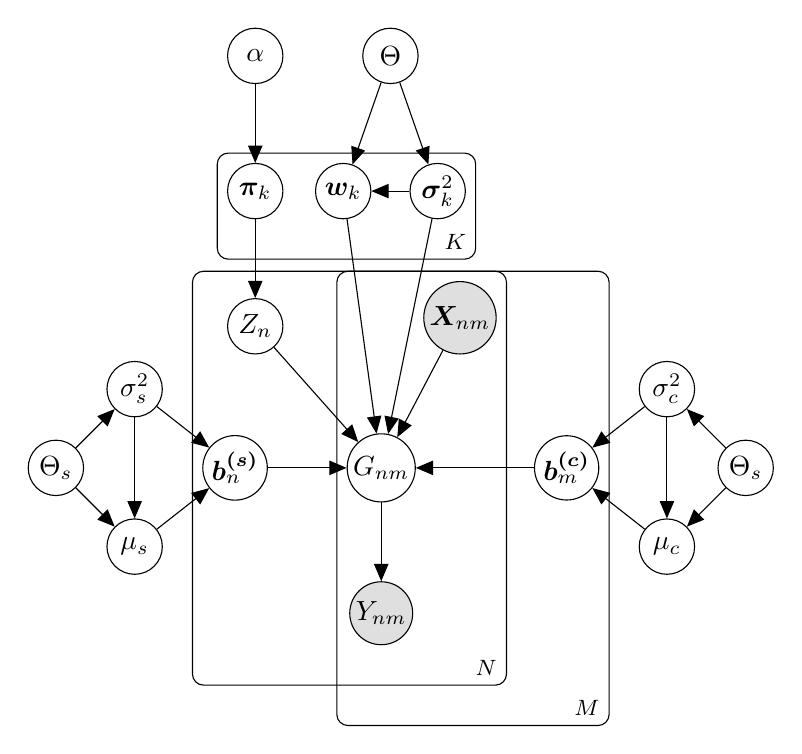
\begin{tikzpicture}

    % Define nodes
    \node[latent]                             (G) {$G_{nm}$};
    \node[obs, below=of G]                    (Y) {$Y_{nm}$};
    \node[obs, above=of G, xshift=1cm]                    (X) {$\bm{X}_{nm}$};
    \node[latent, above=of G, xshift=-1.6cm]    (Z) {$Z_n$};

    \node[latent, above=of Z]                (pi) {$\bm{\pi}_k$};
    \node[latent, above=of pi]            (alpha) {$\alpha$};
    \node[latent, right=of alpha] (theta) {$\Theta$};

    \node[latent, right=of G, xshift=0.5cm]                 (bc) {$\bm{b^{(c)}}_m$};
    \node[latent, right=of bc, xshift=-0.5cm, yshift=1cm]   (sc) {$\sigma_c^2$};
    \node[latent, right=of bc, xshift=-0.5cm, yshift=-1cm]  (mc) {$\mu_c$};
    \node[latent, right=of bc, xshift=0.5cm]            (thetac) {$\Theta_s$};

    \node[latent, left=of G]                                (bs) {$\bm{b^{(s)}}_n$};
    \node[latent, left=of bs, xshift=0.5cm, yshift=1cm]     (ss) {$\sigma_s^2$};
    \node[latent, left=of bs, xshift=0.5cm, yshift=-1cm]    (ms) {$\mu_s$};
    \node[latent, left=of bs, xshift=-0.5cm]            (thetas) {$\Theta_s$};

    \node[latent, below=of theta, xshift=-0.6cm] (mk) {$\bm{w}_k$};
    \node[latent, below=of theta, xshift=0.6cm]  (sk) {$\bm{\sigma}_k^2$};

    % Connect the nodes
    \edge {Z,X,mk,sk} {G};
    \edge {G} {Y};
    \edge {pi} {Z};
    \edge {alpha} {pi};

    \edge {sk} {mk};
    \edge {theta} {mk,sk};

    \edge {thetac} {sc,mc};
    \edge {sc} {mc};
    \edge {sc,mc} {bc};
    \edge {bc} {G};

    \edge {thetas} {ss,ms};
    \edge {ss} {ms};
    \edge {ss,ms} {bs};
    \edge {bs} {G};

    % Plates
    \plate {student} {(Z)(X)(G)(Y)(bs)} {$N$};
    \plate {course}%
           {(X)(G)(Y)(bc)(student.south east)}%
           {$M$};
    \plate {comps} {(pi)(mk)(sk)} {$K$};

  \end{tikzpicture}}
\end{figure}

This model shares the problem of all finite mixture models: how do we select the
optimal number of mixture components $K$? We can bypass this problem by
replacing our Dirichlet prior with a Dirichlet process (DP) prior. The Dirichlet
process is a distribution over distributions, allowing us to represent a
countably infinite mixture of linear regressions. The DP has concentration
parameter $\alpha$ and base distribution $H_0$. So we replace (4-7) above with:
%
\begin{align}
    \pi | H &\sim H  \\
    H | H_0, \alpha &\sim DP(H_0, \alpha)  \\
    H_0 | \Theta &\sim \mathcal{N}\left(
        \beta_0, \frac{1}{\kappa_0} \Sigma_k
    \right) \times IW(\nu_0, \Sigma_0) \\
    \beta_k, \Sigma_k &\sim H_0
\end{align}


% Infinite model.
\begin{figure}[tbh]
  \centering
  \setlength{\belowcaptionskip}{15pt plus 3pt minus 2pt}
  \caption{Infinite Bayesian Mixture of Linear Regressions. The hyper-parameters
           $\Theta = (\beta_0, \kappa_0, \nu_0, \Sigma_0)$}
  \label{fig:infinite-bpmlr}
  \resizebox{0.9\columnwidth}{!}{
  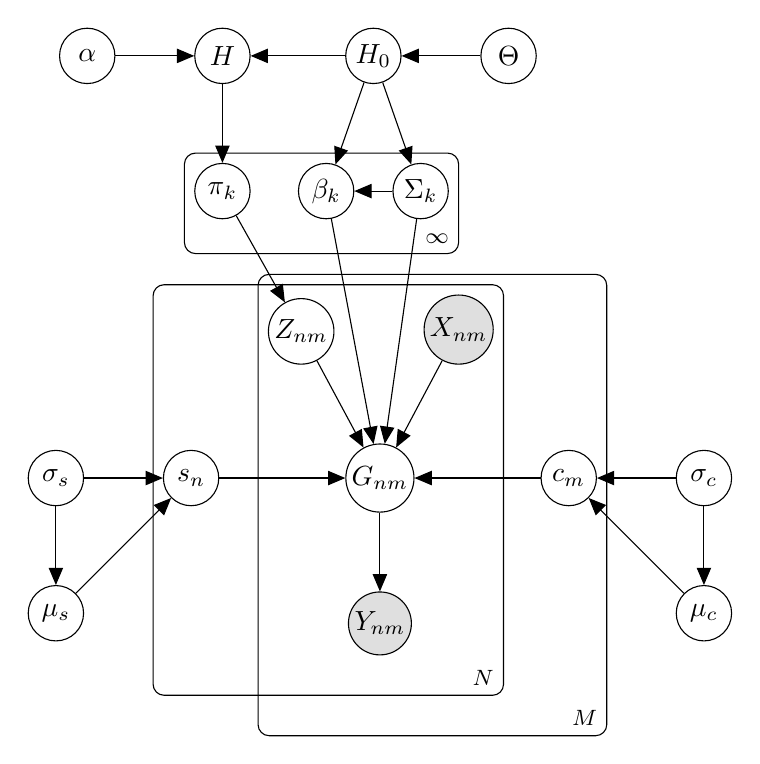
\begin{tikzpicture}

    % Define nodes
    \node[obs]                                (Y) {$Y_{nm}$};
    \node[latent, above=of Y]                 (G) {$G_{nm}$};
    \node[latent, above=of G, xshift=-1cm]    (Z) {$Z_{nm}$};
    \node[obs, above=of G, xshift=1cm]        (X) {$X_{nm}$};

    \node[latent, left=of G, xshift=-0.6cm]   (s) {$s_n$};
    \node[latent, left=of s]                  (ss) {$\sigma_s$};
    \node[latent, below=of ss]                (ms) {$\mu_s$};

    \node[latent, right=of G, xshift=0.6cm]   (c) {$c_m$};
    \node[latent, right=of c]                 (sc) {$\sigma_c$};
    \node[latent, below=of sc]                (mc) {$\mu_c$};

    \node[latent, above=of Z, xshift=-1cm]    (pi) {$\pi_k$};

    \node[latent, above=of pi]                (H) {$H$};
    \node[latent, left=of H]                  (alpha) {$\alpha$};
    \node[latent, right=of H, xshift=0.2cm]   (H0) {$H_0$};
    \node[latent, right=of H0]                (theta) {$\Theta$};

    \node[latent, below=of H0, xshift=-0.6cm] (beta) {$\beta_k$};
    \node[latent, below=of H0, xshift=0.6cm]  (sk) {$\Sigma_k$};

    % Connect the nodes
    \edge {G} {Y};
    \edge {s,c,Z,X,beta,sk} {G};
    \edge {ss,ms} {s};
    \edge {ss} {ms};
    \edge {sc,mc} {c};
    \edge {sc} {mc};

    \edge {pi} {Z};
    \edge {sk} {beta};
    \edge {H} {pi};
    \edge {alpha} {H};
    \edge {H0} {H,beta,sk};
    \edge {theta} {H0};

    % Plates
    \plate {student} {(s)(Z)(X)(G)(Y)} {$N$};
    \plate {course} {(c)(Z)(X)(G)(Y)(student.south east)(student.north east)} {$M$};
    \plate {comps} {(pi)(beta)(sk)} {$\infty$};

  \end{tikzpicture}}
\end{figure}

\cite{gaffney_trajectory_1999},
\cite{gorur_dirichlet_2010},
\cite{kamper_gibbs_2013},
\cite{kottas_nonparametric_2005},
\cite{neal_markov_2000},
\cite{rasmussen_infinite_1999}

\section{Experiments}\label{experiments}

\section{Analysis}\label{analysis}

\section{Previous work}\label{previous work}

\section{Conclusions}\label{conclusions}
We worked hard, and achieved very little.

% use section* for acknowledgement
\section*{Acknowledgment}
This research was funded by NSF IIS grant 1447489.


\bibliographystyle{siam}
\bibliography{dpmlr-refs}

\end{document}

